\newcommand{\expectation}[1]{E[#1]}
\newcommand{\prb}[1]{\mathtt{Prob}~[#1]}

\chapter{Randomized SAT Solvers}
In this chapter we will look at randomized algorithms for propositional formulas. In the first section, we give a polynomial time algorithm for checking satisfiability for 2-CNF formulas. Then we give an exponential time algorithm checking satisfiability for 3-CNF formulas. This algorithm will be better than the trivial $O(2^n)$ algorithm of going through all the assignments to the $n$ propositions. You will observe that both the algorithms are easy to describe. The difficult part is proving that the algorithm answers correctly with ``high" probability. 

\section{$2$-CNF}
The algorithm is given in Algorithm \ref{alg:randtwocnf}. In the algorithm the number of times the loop needs to be iterated (i.e. $m$) will be fixed later depending on the confidence in the algorithm the user requires.

\begin{algorithm}
 \caption{$2$-CNF Satisfiability}
 \label{alg:randtwocnf}
 \begin{algorithmic}[1]
 \renewcommand{\algorithmicrequire}{\textbf{Input:}}
 \renewcommand{\algorithmicensure}{\textbf{Output:}}
 \REQUIRE A $2$-CNF formula $\alpha$
 \ENSURE  $\alpha$ is satisfiable or not.
 \STATE Start with an arbitrary truth assignment.
 \FOR {$m$ steps} 
 \IF {assignment makes $\alpha$ true}
 \STATE Return SAT
 \ENDIF
 \STATE Choose a clause not satisfiable.
 \STATE Choose uniformly at random one of the propositions in the clause and change its assignment.
 \ENDFOR
 \STATE Return UNSAT.
 \end{algorithmic} 
 \end{algorithm}
 
The following claim is an easy observation about the algorithm. 
\begin{lemma}
If the formula $\alpha$ is unsatisfiable then Algorithm \ref{alg:randtwocnf} returns UNSAT. Contra positively, if the algorithm returns SAT, then the formula is satisfiable.
\end{lemma}

Due to the above lemma, the important question we need to answer is, if the formula is satisfiable, how often will the algorithm return UNSAT. That is, what is the probability that the algorithm fails. So, let us assume that the formula is satisfiable and try to answer how long will the algorithm take to return SAT. This will help us in deciding what is a good value for $m$.  

We now try to estimate the expected running time of the algorithm, assuming the formula is satisfiable and the loop runs for ever (i.e $m= \infty$). Let $S$ be a satisfying assignment for $\alpha$. We will try to find the expected running time for finding $S$. Note that, there may be other satisfying assignments and the algorithm might find them before it finds $S$. Therefore, the expected running time we find is a worst case estimate. Consider the $i^{th}$ iteration of the loop. We define $A_i$ and $X_i$ as follows
\[
A_i = \text{ the assignment at the beginning of the }i^{th} \text{ iteration of the loop} 
\]
\[
X_i = \text{ the number of variables whose assignments in } A_i \text{ differ from that of }S
\]

We can try to understand some properties of $X_i$. Note that if $X_i = n$, then all assignments to variables in $A_i$ differ from $S$. The algorithm therefore will find a clause which is not satisfiable. In that clause, assignments to both the propositions are wrong and hence no matter which proposition we pick and change the assignment we get that $X_{i+1}=n-1$.
\[
\prb{X_{i+1} = n-1 ~|~ X_i = n} = 1
\]
Let us now move on to the general case when $X_i = k<n$. We are interested in identifying the probability of $X_{i+1} = k-1$. Let us analyse our algorithm. We have $k$ assignments differing from $S$ and our algorithm picks a clause which is not satisfiable. Atleast one of the proposition in this clause is assigned a truth value in $A_i$ which is different from that in $S$ (note that, it could happen that both the propositions are assigned differently). Our algorithm picks one of the two proposition with equal probability and changes its assignment. Therefore, we pick a proposition whose value is different with probability greater than or equal to $\frac{1}{2}$. If both the propositional values are different we pick with probability $1$. Otherwise we pick with probability $\frac{1}{2}$. Therefore
\[
\prb{X_{i+1} = k-1 ~|~ X_i = k} \geq \frac{1}{2}
\]
A similar analysis also gives us
\[
\prb{X_{i+1} = k+1 ~|~ X_i = k} \leq \frac{1}{2}
\]

Our current understanding is captured by the following set of equations and in Figure \ref{fig:twocnfwalk}.
\begin{equation}
\label{eq:twoexactcnf}
\begin{split}
\prb{X_{i+1} = n-1 ~|~ X_i = n} = 1 \\
\prb{X_{i+1} = k-1 ~|~ X_i = k} \geq \frac{1}{2} ~, \forall k, \text{ where } 0< k < n\\
\prb{X_{i+1} = k+1 ~|~ X_i = k} \leq \frac{1}{2}~, \forall k, \text{ where } 0< k < n
\end{split}
\end{equation}
Let us assume that when we enter the first loop, we have an assignment such that $X_1 = k$. We are interested in finding out how many steps $m$ are required such that $X_m = 0$. Note that, at any iteration of the loop, we can go right one step in the figure (towards $n$) with probability greater than or equal to half and we can move left (towards $0$) with probability, less than or equal to half.

\begin{SCfigure}[1][h]
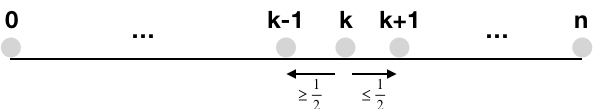
\includegraphics[width=0.5\textwidth]{twocnfwalk}
\caption{At each loop iteration, the algorithm walks one step towards the left or right with probability $\geq \frac{1}{2}$ or $\leq \frac{1}{2}$ respectively.}
\label{fig:twocnfwalk}
\end{SCfigure}

The walk given by Equation \ref{eq:twoexactcnf} is difficult to analyse and therefore we analyse a ``pessimistic" version of the above probability distribution. The equations in this version are approximated by a ``Markov chain" as follows (see also Figure \ref{fig:twoapproxcnfwalk}).
\begin{equation}
\label{eq:twocnf}
\begin{split}
\prb{X_{i+1} = n-1 ~|~ X_i = n} = 1 \\
\prb{X_{i+1} = k-1 ~|~ X_i = k} = \frac{1}{2} ~, \forall k, \text{ where } 0< k < n\\
\prb{X_{i+1} = k+1 ~|~ X_i = k} = \frac{1}{2}~, \forall k, \text{ where } 0< k < n
\end{split}
\end{equation}

\begin{SCfigure}[1][h]
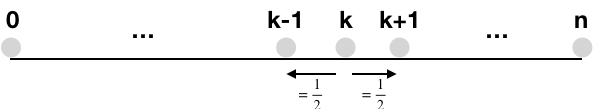
\includegraphics[width=0.5\textwidth]{twoapproxcnfwalk}
\caption{Markov Chain approximation: At each loop iteration, the algorithm walks one step towards the left or right with probability exactly $\frac{1}{2}$. This is a worst case scenario for our algorithm.}
\label{fig:twoapproxcnfwalk}
\end{SCfigure}

Note that, in the former setting, the probability of going left at any point was greater or equal to in the latter setting. Therefore, the probability of reaching $0$ in $m$ number of steps is greater in the former than in the latter. Therefore, the expected number of steps to reach $0$ from $k$ using these set of equations is greater than what we had before. We will give an upperbound for these sets of equations. 

Let $k$ be such that $0 \leq k \leq n$. We will denote by $Z_k$, the random variable representing the number of steps from $k$ to $0$. We are interested in the expected value of $Z_n$ (denoted by 
 $\expectation{Z_n}$). The Equations \ref{eq:twocnf} gives us the following
\begin{equation}
\label{eq:twocnfexpectation}
\begin{split}
\expectation{Z_0} = 0 \\
\expectation{Z_n} = 1 + \expectation{Z_{n-1}} \\
 \forall ~0<k<n, ~\expectation{Z_k} = \frac{1}{2} (1+\expectation{Z_{k-1}}) + \frac{1}{2}(1+\expectation{Z_{k+1})} \\
  = 1 + \frac{1}{2} (\expectation{Z_{k-1}} + \expectation{Z_{k+1}}) 
\end{split}
\end{equation} 

This contains $n+1$ equations on $n+1$ variables. The following claim holds for equations \ref{eq:twocnfexpectation}.
\begin{lemma}
For all $k$, where $0\leq k < n$ we have $\expectation{Z_k} = 2nk-k^2$
\end{lemma}
\begin{proof}
The proof is by induction on $k$. It is easy to observe that the claim holds for the base case $k=0$. Let us assume it true for some $k$ and show that it holds for $k+1$. We know the following
\[
\expectation{Z_k} = 1 + \frac{1}{2} (\expectation{Z_{k-1}} + \expectation{Z_{k+1}}) 
\]
Therefore, the lemma holds due to the following analysis
\begin{align*}
\expectation{Z_{k+1}} & = 2 \big(\expectation{Z_k} - 1 \big) - \expectation{Z_{k-1}} \\
& = 2 (2nk- k^2 -1 ) -  \big( 2n (k-1) - (k-1)^2 \big)  \\
& = 2 (2nk - k^2 -1 ) - \big( 2nk - 2n - (k^2 -2k + 1) \big) \\
& = 2nk - k^2 -1 + 2n - 2k \\
& = 2n(k+1) - (k+1)^2 
\end{align*}
\end{proof}

From this, we get that 
\[
\expectation{Z_n} = 1 + 2n (n-1) - (n-1)^2 = n^2
\]
In other words, the expected number of steps required from any position $k$ to $0$ is less than or equal to $n^2$. This proves the following.
\begin{lemma}
If a $2$-CNF formula is satisfiable, then the algorithm \ref{alg:randtwocnf} outputs SAT in an expected running time of at most $n^2$. 
\end{lemma}

With the above lemma, we can derive a ``good" value for $m$. We show that, if $m=2n^2t$, then the algorithm answers correctly with a probability greater than or equal to $(1 - \frac{1}{2^t})$. 
\begin{theorem}
Let $m = 2n^2t$. Then Algorithm \ref{alg:randtwocnf}. fails with probability less than or equal to $\frac{1}{2^t}$.
\end{theorem}
\begin{proof}
We know that if the formula is not satisfiable, the algorithm does not fail. So, let us assume that the formula is satisfiable. Let $Z$ be the random variable representing the number of steps taken to output SAT. Applying Markov's inequality to the above lemma gives us
\[
\prb{Z \geq 2n^2}  \leq \frac{1}{2}
\]
Let us consider our algorithm as running $t$ loops with each loop running $2n^2$ times. Then, an inside loop fails with probability less than or equal to half. Hence, the probability of the algorithm failing $t$ times is given by the union bound as 
\[
\prb{\text{ algorithm fails }} \leq \frac{1}{2^t}
\]


\end{proof}

\section{$3$-CNF}
Our algorithm will be a modification of the $2$-CNF algorithm. What could go wrong if we applied the same algorithm for the $3$-CNF case. The Markov chain for a $3$-CNF formula is given in Figure \ref{fig:threecnfwalk}. Exercise \ref{ex:threecnf} shows that the expected running time for this algorithm is $O(2^n)$. This is not good enough, since even going through all possible solutions takes only this much time. 

\begin{SCfigure}[1][h]
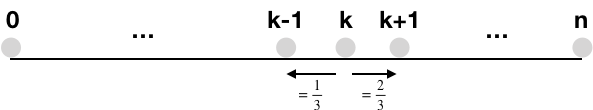
\includegraphics[width=0.5\textwidth]{threecnfwalk}
\caption{Markov Chain approximation: At each loop iteration, the algorithm walks one step towards the left or right with probability $\frac{1}{3}$, and $\frac{2}{3}$ respectively. This is a worst case scenario for our algorithm.}
\label{fig:threecnfwalk}
\end{SCfigure}

We modify our algorithm as follows.
\begin{algorithm}
 \caption{$3$-CNF Satisfiability}
 \label{alg:randthreecnf}
 \begin{algorithmic}[1]
 \renewcommand{\algorithmicrequire}{\textbf{Input:}}
 \renewcommand{\algorithmicensure}{\textbf{Output:}}
 \REQUIRE A $3$-CNF formula $\alpha$
 \ENSURE  $\alpha$ is satisfiable or not.
 \FOR {$m$ steps}
	 \STATE Start with an arbitrary truth assignment.
	 \FOR {$3n$ steps} 
		 \IF {assignment makes $\alpha$ true}
			 \STATE Return SAT
		 \ENDIF			 
		 \STATE Choose a clause not satisfiable.
		 \STATE Choose uniformly at random one of the propositions in the clause and change its assignment.
 	\ENDFOR
 \ENDFOR
 \STATE Return UNSAT.
\end{algorithmic} 
\end{algorithm}

As in the $2$-CNF algorithm, we know that if the formula is unsatisfiable, then the algorithm will return UNSAT. Let us now calculate the expected running time of the algorithm if $m=\infty$ and assuming the formula is satisfiable. Like in the previous analysis, let $S$ be the satisfying assignment. Let us now consider the run of an outer loop. We start from an arbitrary assignment for $\alpha$.  For the $i^{th}$ iteration of the inner loop we denote by $A_i$ the assignment at the beginning of the inner loop. We want to bound the probability that the $3n$ steps of the inner loop does not identify the satisfying assignment. Let us assume that the after the initial arbitrary assignment, $k$ many propositions are wrongly assigned. Let us denote by $q_k$ the probability that we reach a satisfying assignment within $3n$ steps of the inner loop. That is, the probability of reaching $0$ from $k$ by doing a random walk on the Markov Chain given in Figure \ref{fig:threecnfwalk}. Note that, in the special case of $k=0$, we have $q_0 = 1$. For a general $k>0$, there is no bound on the number of left or right moves required to reach $0$. Let us consider, a special case when the number of right moves is $k$ and the number of left moves is $2k$. Clearly $q_k$ is greater than the probability of this happening. Thus
\[
q_k \geq {3k \choose k} \big(\frac{1}{3}\big)^{2k} \big( \frac{2}{3} \big)^k
\]

Stirling's formula gives that there are constants $c_1$ and $c_2$ such that for any $n>0$, we have $c_1 \sqrt{n} \big(\frac{n}{e}\big)^n \leq n! \leq  c_2 \sqrt{n} \big(\frac{n}{e}\big)^n$. This can now be used to find a better bound for $q_k$.
\begin{align*}
q_k & \geq \frac{3k!}{k!}{2k!} \big(\frac{1}{3}\big)^{2k} \big( \frac{2}{3} \big)^k \\
& \geq \frac{c_1\sqrt{3k} (\frac{3k}{e})^{3k}}{c_2 \sqrt{k} (\frac{k}{e})^k c_2 \sqrt{2k} (\frac{2k}{e})^{2k}} \big(\frac{1}{3}\big)^{2k} \big( \frac{2}{3} \big)^k \\
& \geq c \frac{1}{\sqrt{k}} \frac{1}{2^k} \text{  , for a constant } c
\end{align*}

We now have a bound on $q_k$. Let us now calculate the probability $q$ that we find the satisfying assignment given that we start from a random assignment. Then,
\begin{align*}
q & = \sum_{k=0}^n \prb{\text{assignment to exactly $k$ propositions are different from that of } S ~} \times q_k \\
& \geq \frac{1}{2^n} + \sum_{k=1}^n {n \choose k} \frac{1}{2^n}  \frac{c}{\sqrt{k}} \frac{1}{2^k} \\
& \geq \frac{1}{2^n} \frac{c}{\sqrt{n}} + \sum_{k=1}^n {n \choose k} \frac{1}{2^n}  \frac{c}{\sqrt{n}} \frac{1}{2^k} \\
& = \frac{c}{\sqrt{n}2^n} \sum_{k=0}^n {n \choose k}  \frac{1}{2^k}  \\
& = \frac{c}{\sqrt{n}2^n} (1 + \frac{1}{2})^n ~(\text{ using the expansion for } (1 + \frac{1}{2})^n ) \\
& = \frac{c}{\sqrt{n}} \big(\frac{3}{4}\big)^n 
\end{align*}

Thus the probability of success starting from an arbitrary assignment and walking $3n$ steps is $\geq \frac{c}{\sqrt{n}} \big(\frac{3}{4}\big)^n$. Thus the expected running time of the outer loop for success is given by 
\[
O(\sqrt{n} \big(\frac{4}{3}\big)^n)
\]
Let $a$ be denoted by this number. Thus the total number of steps of the algorithm is $a \times 3n$. We will now show that taking $m = 2at$ will ensure that the probability of failure of our algorithm is less than or equal to $\frac{1}{2^t}$. 
\begin{theorem}
Let $a = \frac{\sqrt{n}}{c} \big(\frac{4}{3}\big)^n)$ and $m = 2at$. Then the running time of Algorithm \ref{alg:randthreecnf}. is $O(n^{\frac{3}{2}}\big(\frac{4}{3}\big)^n)$ and the probability of failure is less than or equal to $\frac{1}{2^t}$. 
\end{theorem}
\begin{proof}
The running time of the algorithm is $3n \times \frac{\sqrt{n}}{c} \big(\frac{4}{3}\big)^n) = O(n^{\frac{3}{2}}\big(\frac{4}{3}\big)^n)$. The algorithm will fail only if the formula is satisfiable. Let $Z$ be the random variable denoting the number of outer loops required for finding the satisfying assignments. Using Markov's inequality we can show that
\[
\prb{Z \geq 2a} \leq \frac{1}{2}
\]
Let us again consider that we are running the algorithm $t$ times and each time we are running the outer loop for $2a$ times. Thus the probability of failure for all the $t$ times is given by the union bound by
\[
\prb {\text{algorithm fails }} \leq \frac{1}{2^t}
\]

\end{proof}


